\documentclass{article}
\usepackage[utf8]{inputenc}

\documentclass[a4paper]{article}
\usepackage[12pt]{extsizes}
\usepackage{amsmath,amsthm,amssymb}
\usepackage[hidelinks]{hyperref} 
\usepackage[warn]{mathtext}
\usepackage[T1,T2A]{fontenc}
\usepackage[utf8]{inputenc}
\usepackage[english,russian]{babel}
\usepackage{tocloft}
\linespread{1.5}
\usepackage{indentfirst}
\usepackage{setspace}
%\полуторный интервал
\onehalfspacing

\newcommand{\RomanNumeralCaps}[1]
    {\MakeUppercase{\romannumeral #1}}

\usepackage{amssymb}

\usepackage{graphicx, float}
\graphicspath{{pictures/}}
\DeclareGraphicsExtensions{.pdf,.png,.jpg}
\usepackage[left=25mm,right=1cm,
    top=2cm,bottom=20mm,bindingoffset=0cm]{geometry}
\renewcommand{\cftsecleader}{\cftdotfill{\cftdotsep}}

\addto\captionsrussian{\renewcommand{\contentsname}{СОДЕРЖАНИЕ}}
\addto\captionsrussian{\renewcommand{\listfigurename}{СПИСОК ИЛЛЮСТРАЦИЙ}}

\usepackage{fancyhdr}
\usepackage[nottoc]{tocbibind}

\fancypagestyle{plain}{
\fancyhf{}
\renewcommand{\headrulewidth}{0pt}
\fancyhead[R]{\thepage}
}

\usepackage{blindtext}
\pagestyle{myheadings}
\usepackage{hyperref}

\begin{document}
\begin{titlepage}
  \begin{center}
    \large
    Санкт-Петербургский политехнический университет Петра Великого
    
    Институт прикладной математики и механики
    
    \textbf{Высшая школа прикладной математики и вычислительной физики}
    \vfill
    \textsc{\textbf{\Large{Отчёт по лабораторной работе №6}}}\\[5mm]
    \\ по дисциплине
    \\ <<Математическая статистика>>\\
\end{center}

\vfill

\begin{tabular}{l p{140} l}
Выполнил студент \\группы 3630102/80401 && Веденичев Дмитрий Александрович \\
\\
Проверил\\Доцент, к.ф.-м.н.& \hspace{0pt} &   Баженов Александр Николаевич \\\\
\end{tabular}

\hfill \break
\hfill \break
\begin{center} Санкт-Петербург \\2021 \end{center}
\thispagestyle{empty}
\end{titlepage}
\newpage
\newpage
\begin{center}
    \setcounter{page}{2}
    \tableofcontents
\end{center}
\newpage
\begin{center}
    \setcounter{page}{3}
    \listoffigures
\end{center}

\newpage
\section{Постановка задачи}
\noindent Найти оценки коэффициентов линейной регрессии $y_{i} = a + bx_{i} + e_{i}$, используя 20 точек на отрезке [-1.8; 2] с равномерным шагом равным 0.2. Ошибку $e_{i}$ считать нормально распределённой с параметрами (0, 1). В качестве эталонной зависимости взять $y_{i} = 2 + 2x_{i} + e_{i}$. При построении оценок коэффициентов использовать два критерия: критерий наименьших квадратов и критерий наименьших модулей. Проделать то же самое для выборки, у которой в значения $y_{1}$ и $y_{20}$ вносятся возмущения 10 и -10. 

\section{Теория}
\subsection{Простая линейная регрессия}
	\subsubsection{Модель простой линейной регрессии}
	\noindent Регрессионную модель описания данных называют простой линейной регрессией, если
	\begin{equation}
	    y_{i} = \beta_{0} + \beta_{1}x_{i} + \varepsilon_{i},  i = 1..n
	    \label{y_i}
	\end{equation}

	\noindent где $x_1,...,x_n - $ заданные числа (значения фактора);
	$y_1,...y_n - $ наблюдаемые значения отклика;
	$\varepsilon_1,...,\varepsilon_n - $ независимые, нормально распределенные $N(0, \sigma)$ с нулевым математическим ожиданием и одинаковой (неизвестной) дисперсией случайные величины (ненаблюдаемые);
	$\beta_0, \beta_1 - $ неизвестные параметры, подлежащие оцениванию.
	
    \noindent В модели (\ref{y_i}) отклик y зависит зависит от одного фактора x, и весь разброс экспериментальных точек объясняется только погрешностями наблюдений (результатов измерений) отклика y. Погрешности результатов измерений x в этой модели полагают существенно меньшими погрешностей результатов измерений y, так что ими можно пренебречь [1, с. 507].

	\subsubsection{Метод наименьших квадратов}
	\noindent При оценивании параметров регрессионной модели используют различные методы. Один из наиболее распрстранённых подходов заключается в следующем: вводится мера (критерий) рассогласования отклика и регрессионной функции, и оценки параметров регрессии определяются так, чтобы сделать это рассогласование наименьшим. Достаточно простые расчётные формулы для оценок получают при выборе критерия в виде суммы квадратов отклонений значений отклика от значений регрессионной функции (сумма квадратов остатков):
	\begin{equation}
	    Q(\beta_{0}, \beta_{1}) = \sum_{i=1}^{n}{\varepsilon_{i}^{2}} = 
	    \sum_{i=1}^{n}{(y_{i} - \beta_{0} - \beta_{1}x_{i})^{2}}\rightarrow \min_{\beta_{0}, \beta_{1}}
	    \label{Q_beta}
	\end{equation}
	Задача минимизации квадратичного критерия $Q(\beta_0, \beta_1)$ носит название задачи метода наименьших квадратов (МНК), а оценки $\hat{\beta_0}, \hat{\beta_1}$ параметров $\beta_0, \beta_1$, реализующие минимум критерия $Q(\beta_0, \beta_1)$, называют МНК-оценками [1, с. 508]. 

	\subsubsection{Расчётные формулы для МНК-оценок}
	\noindent МНК-оценки параметров $\hat{\beta_0}, \hat{\beta_1}$ находятся из условия обращения функции $Q(\beta_0, \beta_1)$ в минимум. 
	\newline
	Для нахождения МНК-оценок $\hat{\beta_0}, \hat{\beta_1}$ выпишем необходимые условия экстремума
	\begin{equation}
	   \begin{cases}
         & \frac{\partial Q}{\partial \beta_{0}}  = 
         -2\sum_{i=1}^{n}{(y_{i} - \beta_{0} - \beta_{1}x_{i})} = 0\\ 
         & \frac{\partial Q}{\partial \beta_{1}}  = 
         -2\sum_{i=1}^{n}{(y_{i} - \beta_{0} - \beta_{1}x_{i})x_{i}} = 0 
       \end{cases}
       \label{sys_min}
	\end{equation}
	Далее для упрощения записи сумм будем опускать индекс суммирования. Из системы (\ref{sys_min}) получим:
	\begin{equation}
	   \begin{cases}
         & n\hat{\beta_{0}} + \hat{\beta_{1}}\sum_{}{}{x_{i}} = 
         \sum_{}{}{y_{i}}\\ 
        & \hat{\beta_{0}}\sum_{}{}{x_{i}} + \hat{\beta_{1}}\sum_{}{}{x_{i}^{2}} = \sum_{}{}{x_{i}y_{i}}
       \end{cases}
       \label{sys_2}
	\end{equation}
	Разделим оба уравнения на n:
	\begin{equation}
	   \begin{cases}
         & \hat{\beta_{0}} + \hat{\beta_{1}}(\frac{1}{n}\sum_{}{}{x_{i}}) = 
         \frac{1}{n}\sum_{}{}{y_{i}}\\ 
        & \hat{\beta_{0}}(\frac{1}{n}\sum_{}{}{x_{i}}) + \hat{\beta_{1}}(\frac{1}{n}\sum_{}{}{x_{i}^{2}}) = \frac{1}{n}\sum_{}{}{x_{i}y_{i}}
       \end{cases}
       \label{sys_3}
	\end{equation}
	и, используя известные статистические обозначения для выборочных первых и вторых начальных моментов
	\begin{equation}
	    \bar{x} = \frac{1}{n}\sum_{}{}{x_{i}}, \bar{y} = \frac{1}{n}\sum_{}{}{y_{i}}, \bar{x^{2}} = \frac{1}{n}\sum_{}{}{x_{i}^{2}}, \bar{xy} = \frac{1}{n}\sum_{}{}{x_{i}y_{i}}, 
	\end{equation}
	получим
		\begin{equation}
	   \begin{cases}
         & \hat{\beta_{0}} + \hat{\beta_{1}}\bar{x} = 
         \bar{y}\\ 
        & \hat{\beta_{0}}\bar{x} + \hat{\beta_{1}}\bar{x^{2}} = \bar{xy},
       \end{cases}
       \label{sys_fin}
	\end{equation}
	откуда МНК-оценку $\hat{\beta_1}$ наклона прямой регрессии находим по формуле Крамера
	\begin{equation}
	    \hat{\beta_{1}} = \frac{\bar{xy} - \bar{x} \cdot \bar{y}}{\bar{x^{2}} - (\bar{x})^{2}}
	    \label{beta_1_new}
	\end{equation}
	a МНК-оценку $\hat{\beta_0}$  определяем непосредственно из первого уравнения системы (\ref{sys_fin}):
	\begin{equation}
	    \hat{\beta_{0}} = \bar{y} - \bar{x}\hat{\beta_{1}}
	    \label{beta_0_new}
	\end{equation}
	Заметим, что определитель системы (\ref{sys_fin}):
	\begin{equation}
	    \bar{x^{2}} - (\bar{x})^{2} = \frac{1}{n}\sum_{}{}{(x_{i} - \bar{x})^{2}} = s_{x}^{2} > 0, 
	\end{equation}
	если среди значений $x_{1},...,x_{n}$ есть различные, что и будем предполагать.
	\newline
	Доказательство минимальности функции $Q(\beta_{0}, \beta_{1})$ в стационарной точке проведём с помощью известного достаточного признака экстремума функции двух переменных. Имеем:
	\begin{equation}
	    \frac{\partial ^{2} Q}{\partial \beta_{0}^{2}} = 2n, 
        \frac{\partial ^{2} Q}{\partial \beta_{1}^{2}} = 2\sum_{}{}{x_{i}^{2}} = 2n\bar{x^{2}}, 
        \frac{\partial ^{2} Q}{\partial \beta_{1} \partial \beta_{0}} = 2\sum_{}{}{x_{i}} = 2n\bar{x}
        \label{frac_eq}
	\end{equation}
	\begin{equation}
	    \bigtriangleup = \frac{\partial^{2}Q}{\partial \beta_{0}^{2}} \cdot \frac{\partial^{2}Q}{\partial \beta_{1}^{2}} - (\frac{\partial^{2}Q}{\partial \beta_{1} \partial \beta_{0}})^{2} = 
	    4n^{2}\bar{x^{2}} - 4n^2(\bar{x})^{2} = 
	    4n^{2}\left[\bar{x^{2}} - (\bar{x})^{2}\right] = 4n^{2}\left[ \frac{1}{n}\sum{}_{}{(x_{i} - \bar{x})}\right] = 4n^{2}s_{x}^{2} > 0.
	    \label{det_sys}
	\end{equation}
	Этот результат вместе с условием $\frac{\partial^{2}Q}{\partial \beta_{0}^{2}} = 2n > 0$ означает, что в стационарной точке функция Q имеет минимум [1, с. 508-511].




	
	


    \subsection{Робастные оценки коэффициентов линейной регрессии}
    \noindent Робастность оценок коэффициентов линейной регрессии (т.е. их устойчивость по отношению к наличию в данных редких, но больших по величине выбросов) может быть обеспечена различными способами. Одним из них является использование метода наименьших модулей вместо метода наименьших квадратов:
    \begin{equation}
	    \sum_{i=1}^{n}{|y_{i} - \beta_{0} - \beta_{1}x_{i}|}\rightarrow \min_{\beta_{0}, \beta_{1}}
	    \label{min_abs}
	\end{equation}
    Напомним, что использование метода наименьших модулей в задаче оценивания параметра сдвига распределений приводит к оценке в виде выборочной медианы, обладающей робастными свойствами. В отличие от этого случая и от задач метода наименьших квадратов, на практике задача (\ref{min_abs}) решается численно. Соответствующие процедуры представлены в некоторых современных пакетах программ по статистическому анализу.
    \newline
    Здесь мы рассмотрим простейшую в вычистлительном отношении робастную альтернативу оценкам коэффициентов линейной регрессии по МНК. Для этого сначала запишем выражения для оценок (\ref{beta_0_new}) и (\ref{beta_1_new}) в другом виде:
    \begin{equation}
    	\begin{cases}
        \hat{\beta_{1}} = \frac{\bar{xy} - \bar{x} \cdot \bar{y}}{\bar{x^{2}} - (\bar{x})^{2}} = \frac{k_{xy}}{s_{x}^{2}} = \frac{k_{xy}}{s_{x}s_{y}} \cdot \frac{s_{y}}{s_{x}} = r_{xy}\frac{s_{y}}{s_{x}} \\         
        \hat{\beta_{0}} = \bar{y} - \bar{x}\hat{\beta_{1}}
        \end{cases}
        \label{new_coef_abs}
    \end{equation}
    В формулах (\ref{new_coef_abs}) заменим выборочные средние $\bar{x}$ и $\bar{y}$ соответственно на робастные выборочные медианы $med x$ и $med y$, среднеквадратические отклонения $s_{x}$ и $s_{y}$ на робастные нормированные интерквартильные широты $q^{*}_{x}$ и $q^{*}_{y}$, выборочный коэффициент корреляции $r_{xy}$ — на знаковый коэффициент корреляции $r_{Q}$: 
    \begin{equation}
        \hat{\beta_{1}}_{R} = r_{Q}\frac{q^{*}_{y}}{q^{*}_{x}},
        \label{b_1R}
    \end{equation}
    \begin{equation}
        \hat{\beta_{0}}_{R} = med y - \hat{\beta_{1}}_{R} med x,
        \label{b_0R}
    \end{equation}
    \begin{equation}
        r_{Q} = \frac{1}{n}\sum_{i=1}^{n}{sgn(x_{i} - med x)sgn(y_{i} - med y)},
        \label{r_Q}
    \end{equation}
    \begin{multline}
    \\
        q^{*}_{y} = \frac{y_{(j)} -y_{(l)}}{k_{q}(n)},~~~
        q^{*}_{x} = \frac{x_{(j)} - x_{(l)}}{k_{q}(n)}, \\ 
        \begin{cases}
             & [\frac{n}{4}] + 1 \text{ при } \frac{n}{4} \text{ дробном, } \\ 
             & \frac{n}{4} \text{ при } \frac{n}{4} \text{ целом. }
        \end{cases}\\
        j = n - l + 1\\
        sgn(z) = \begin{cases}
                    & 1 \text{ при } z > 0 \\ 
                    & 0 \text{ при } z = 0 \\
                    & -1 \text{ при } z < 0
                 \end{cases}\\
        \label{q*}        
    \end{multline}
    Уравнение регрессии здесь имеет вид 
    \begin{equation}
        y = \hat{\beta_{0}}_{R} +  \hat{\beta_{1}}_{R}x
        \label{y}
    \end{equation}
    Статистики выборочной медианы и интерквартильной широты обладают робастными свойствами в силу того, что основаны на центральных порядковых статистиках, малочувствительных к большим по величине выбросам в данных. Статистика выборочного знакового коэффициента корреляции робастна, так как знаковая функция $sgn z$ чувствительна не к величине аргумента, а только к его знаку. Отсюда оценка прямой регрессии (\ref{y}) обладает очевидными робастными свойствами устойчивости к выбросам по координате y, но она довольно груба [1, с. 518-519].
    
    \section{Программная реализация}
    \noindent Лабораторная работа выполнена на языке Python вресии 3.7 в среде разработки JupyterLab. Использовались дополнительные библиотеки:
 \begin{enumerate}
        \item scipy
        \item matplotlib
        \item numpy 
    \end{enumerate}
В приложении находится ссылка на GitHub репозиторий с исходныи кодом.

\section{Результаты}
\subsection{Оценки коэффициентов линейной регрессии}
	
	\noindent Метрика удаленности: $dist = \sum_{i=0}^{n}(y_{model}[i]-y_{regr}[i])^2$
	\subsubsection{Выборка без возмущений}
		\begin{enumerate}
			\item{Критерий наименьших квадратов:}
			$\hat{a}\approx 1.67$, $\hat{b}\approx 2.47$
			\item{Критерий наименьших модулей:}
			$\hat{a}\approx 1.44$, $\hat{b}\approx 2.59$
		\end{enumerate}
		\begin{figure}[H]
			\centering
			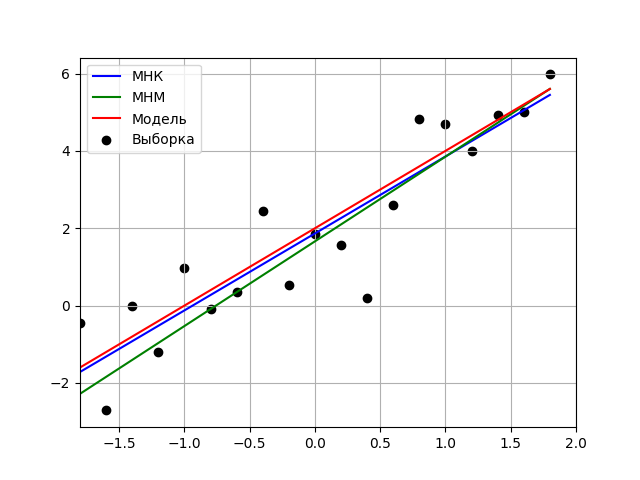
\includegraphics[width = 10cm, height = 8cm]{NoPerturb.png}
			\caption{Выборка без возмущений}
			\label{w/o_pert}
		\end{figure}
		$МНК~dist~=~17.7$ \\
		$МНМ~dist~=~19.0$
	
	\subsubsection{Выборка с возмущениями}
		\begin{enumerate}
			\item{Критерий наименьших квадратов:}
			$\hat{a}\approx 1.95$, $\hat{b}\approx 0.29 $
			\item{Критерий наименьших модулей:}
			$\hat{a}\approx 1.83$, $\hat{b}\approx 0.93$
		\end{enumerate}
		\begin{figure}[H]
			\centering
			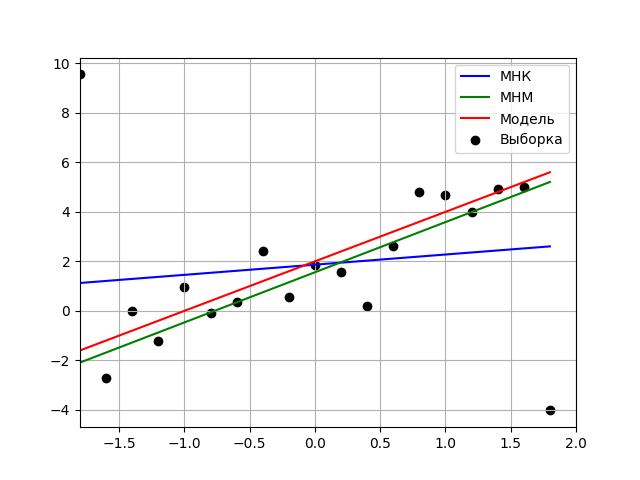
\includegraphics[width = 10cm, height = 8cm]{Perturb.png}
			\caption{Выборка с возмущениями}
			\label{w_pert}
		\end{figure}
		$МНК~dist~=~173.73$ \\
		$МНМ~dist~=~183.49$

\section{Обсуждение}
\subsection{Оценки коэффициентов линейной регрессии}
	
\noindent По полученным результатам можно сказать, что используя критерий наименьших квадратов удастся точнее оценить коэффициенты линейной регрессии для выборки без возмущений. Критерий наименьших модулей устойчив к редким выбросам

\section{Приложение}
\noindent Код программы GitHub URL:\\https://github.com/PopeyeTheSailorsCat/math\_stat\_2021/tree/main/lab6
\newline 


\end{document}
